\upaper{15}{СЕМЬ СВЕРХВСЕЛЕННЫХ}
\uminitoc{ПРОСТРАНСТВЕННЫЙ УРОВЕНЬ СВЕРХВСЕЛЕННЫХ}
\uminitoc{ОРГАНИЗАЦИЯ СВЕРХВСЕЛЕННЫХ}
\uminitoc{СВЕРХВСЕЛЕННАЯ ОРВОНТОН}
\uminitoc{ТУМАННОСТИ --- ПРАРОДИТЕЛИ ВСЕЛЕННЫХ}
\uminitoc{ПРОИСХОЖДЕНИЕ ТЕЛ В ПРОСТРАНСТВЕ}
\uminitoc{СФЕРЫ ПРОСТРАНСТВА}
\uminitoc{АРХИТЕКТУРНЫЕ СФЕРЫ}
\uminitoc{КОНТРОЛЬ И РЕГУЛИРОВАНИЕ ЭНЕРГИИ}
\uminitoc{КОНТУРЫ СВЕРХВСЕЛЕННЫХ}
\uminitoc{ПРАВИТЕЛИ СВЕРХВСЕЛЕННЫХ}
\uminitoc{СОВЕЩАТЕЛЬНАЯ АССАМБЛЕЯ}
\uminitoc{ВЕРХОВНЫЕ СУДЫ}
\uminitoc{ПРАВИТЕЛЬСТВА СЕКТОРОВ}
\uminitoc{ЦЕЛИ СЕМИ СВЕРХВСЕЛЕННЫХ}
\author{Всеобщий Цензор}
\vs p015 0:1 Для Всеобщего Отца --- как для Отца --- вселенные фактически не существуют; он имеет дело с личностями; он является Отцом личностей. Для Вечного Сына и Бесконечного Духа --- как для создателей\hyp{}партнёров --- вселенные представляют собой локализованные и индивидуальные творения, находящиеся под совместным правлением Сынов Создателей и Созидательных Духов. Для Райской Троицы за пределами Хавоны существует всего семь обитаемых вселенных, --- семь сверхвселенных, в юрисдикцию которых входит круг первого уровня пост\hyp{}Хавонского пространства. Семь Главных Духов излучают своё влияние из центрального Острова, делая тем самым огромное творение одним гигантским колесом, центральный стержень которого --- вечный Остров Рай, семь спиц --- излучения Семи Главных Духов, обод --- внешние области большой вселенной.
\vs p015 0:2 В начале материализации всеобщего творения была сформулирована семеричная схема организации и правления сверхвселенными. Первое творение после Хавоны было разделено на семь колоссальных сегментов, и были спроектированы и сконструированы столичные миры для правительств этих сверхвселенных. Нынешняя система управления существует почти от вечности, и правители этих семи сверхвселенных справедливо называются От Века Древними.
\vs p015 0:3 Из огромного объёма знаний о сверхвселенных я могу поведать тебе лишь немногое, но повсюду в этих областях действует метод разумного управления как над физическими, так и над духовными силами, а всеобщие гравитационные присутствия функционируют там с величественной мощью и в совершенной гармонии. Вначале важно получить адекватное представление о физическом устройстве и материальной организации областей сверхвселенных, поскольку тогда ты сможешь лучше усвоить значение изумительной организации, предусмотренной для их духовного управления и интеллектуального развития волевых созданий, живущих на мириадах обитаемых планет, разбросанных по этим семи сверхвселенным.
\usection{ПРОСТРАНСТВЕННЫЙ УРОВЕНЬ СВЕРХВСЕЛЕННЫХ}
\vs p015 1:1 В записях, наблюдениях и воспоминаниях, ограниченных миллионом или миллиардом ваших коротких лет, Урантия и вселенная, к которой она принадлежит, участвуют в приключении долгого и неизведанного устремления в новое пространство; но согласно записям Уверсы, в соответствии с более ранними наблюдениями и в гармонии с более обширным опытом и расчётами нашего уровня, и в результате заключений, основанных на этих и других выводах, мы знаем, что вселенные вовлечены в упорядоченную, хорошо осмысленную и безупречно управляемую процессию, в величественном великолепии кружащуюся вокруг Первого Великого Источника и Центра и вселенной его пребывания.
\vs p015 1:2 Мы давно обнаружили, что семь сверхвселенных обращаются по громадному эллипсу, гигантскому и вытянутому кругу. Ваша солнечная система и другие миры времени отнюдь не устремляются в неизведанное пространство неуправляемо, без карты и компаса. Локальная вселенная, к которой принадлежит ваша система, следует определённым и хорошо осмысленным курсом, двигаясь против часовой стрелки по огромной замкнутой дуге вокруг центральной вселенной. Этот космический путь полностью нанесён на карты и так же хорошо известен сверхвселенским наблюдателям звёзд, как орбиты планет, составляющих вашу солнечную систему, известны астрономам Урантии.
\vs p015 1:3 Урантия расположена в ещё не полностью сформированных как локальной, так и сверхвселенной, и ваша локальная вселенная находится в непосредственной близости от многочисленных частично завершённых физических творений. Вы принадлежите к одной из относительно молодых вселенных. Однако сегодня вы не устремляетесь наугад в неизведанное пространство и не качаетесь слепо в неизвестных регионах. Вы следуете упорядоченным и предусмотренным путём, относящимся к пространственному уровню сверхвселенных. Сейчас вы проходите через то же пространство, которое ваша планетарная система или её предшественники пересекали много веков назад; и когда\hyp{}нибудь в далёком будущем ваша система или её преемники вновь пересекут то же самое пространство, сквозь которое вы сейчас столь стремительно проноситесь.
\vs p015 1:4 \pc В данную эпоху и согласно принятым на Урантии представлениям о направлении, сверхвселенная номер один поворачивается почти строго на север, к востоку от Райской резиденции Великих Источников и Центров и центральной вселенной Хавоны, приблизительно напротив неё. Эта позиция, вместе с соответствующей ей на западе, представляет собой ближайшее физическое приближение сфер времени к вечному Острову. Сверхвселенная номер два расположена на севере, готовясь к повороту в западном направлении, а третья сейчас занимает самый северный сегмент великого пространственного пути, уже повернув в изгиб, ведущий к южному направлению. Номер четыре проходит сравнительно прямой участок полёта в южном направлении, и её передние области теперь приближаются к позиции напротив Великих Центров. Номер пять почти покинула свою позицию напротив Центра Центров, продолжая двигаться прямым курсом на юг, как раз перед поворотом на восток; номер шесть занимает б\'ольшую часть южной дуги, сегмент которой ваша сверхвселенная уже почти прошла.
\vs p015 1:5 Ваша локальная вселенная Небадон принадлежит к Орвонтону --- седьмой сверхвселенной, обращающейся между первой и шестой сверхвселенными, не так давно обогнувшей (согласно нашим представлениям о времени) юго\hyp{}восточный изгиб пространственного уровня сверхвселенных. Сегодня солнечная система, к которой принадлежит Урантия, прошла за несколько предыдущих миллиардов лет поворот вокруг южного изгиба, так что вы только сейчас покидаете юго\hyp{}восточный изгиб и быстро продвигаетесь по длинному и относительно прямому пути в северном направлении. В течение бессчётных веков Орвонтон будет следовать этим почти прямым курсом на север.
\vs p015 1:6 Урантия принадлежит к системе, расположенной недалеко от границы вашей локальной вселенной; а ваша локальная вселенная в настоящее время пересекает периферию Орвонтона. За вами есть ещё другие творения, но вы сильно удалены в пространстве от тех физических систем, которые обращаются по великому кругу в сравнительной близости к Великому Источнику и Центру.
\usection{ОРГАНИЗАЦИЯ СВЕРХВСЕЛЕННЫХ}
\vs p015 2:1 Только Всеобщий Отец знает местонахождение и фактическое число обитаемых миров в пространстве; он называет их всех по имени и номеру. Я могу назвать лишь приблизительное число обитаемых или пригодных для обитания планет, ибо в одних локальных вселенных больше миров, пригодных для разумной жизни, чем в других. Кроме того, ещё не все спроектированные локальные вселенные организованы. Поэтому предлагаемые мной оценки предназначены исключительно для того, чтобы дать некоторое представление о необъятности материального творения.
\vs p015 2:2 \pc Большая вселенная включает семь сверхвселенных, и устроены они приблизительно так:
\vs p015 2:3 \li{1.}\bibemph{Система}. Основная единица сверхуправления состоит примерно из 1000 обитаемых или пригодных для обитания миров. Пылающие солнца, холодные миры, планеты, слишком близко расположенные к горячим солнцам, и другие сферы, не пригодные для обитания созданий, не включены в эту группу. Эти 1000 миров, приспособленных для поддержания жизни, называются системой, однако в более молодых системах лишь сравнительно небольшое количество миров может быть обитаемым. Каждую обитаемую планету возглавляет Планетарный Принц, а каждая локальная система имеет в качестве своей столицы архитектурную сферу, управляемую Властелином Системы.
\vs p015 2:4 \li{2.}\bibemph{Созвездие}. Сто систем (около 100\,000 пригодных для обитания планет) составляют созвездие. Каждое созвездие имеет столичную архитектурную сферу и возглавляется тремя Сынами Ворондадеками, Всевышними. Каждое созвездие находится также под наблюдением От Века Верного, посла Райской Троицы.
\vs p015 2:5 \li{3.}\bibemph{Локальная вселенная}. Сто созвездий (около 10\,000\,000 пригодных для обитания планет) составляют локальную вселенную. Каждая локальная вселенная имеет великолепный архитектурный столичный мир и управляется одним из равных Сынов Создателей Бога категории Михаил. Каждая вселенная благословлена присутствием От Века Единого, представителя Райской Троицы.
\vs p015 2:6 \li{4.}\bibemph{Малый сектор}. Сто локальных вселенных (около 1\,000\,000\,000 пригодных для обитания планет) составляют малый сектор управления сверхвселенной; он имеет прекрасный столичный мир, откуда его правители, От Века Недавние, руководят делами малого сектора. На столичном центре каждого малого сектора находятся трое От Века Недавних, Верховных Троичных Личностей.
\vs p015 2:7 \li{5.}\bibemph{Большой сектор}. Сто малых секторов (около 100\,000\,000\,000 пригодных для обитания миров) составляют один большой сектор. Каждый большой сектор снабжён превосходным центром и возглавляется тремя От Века Совершенными, Верховными Троичными Личностями.
\vs p015 2:8 \li{6.}\bibemph{Сверхвселенная}. Десять больших секторов (около 1\,000\,000\,000\,000 пригодных для обитания планет) составляют сверхвселенную. Каждая сверхвселенная обеспечена огромным и великолепным столичным миром и управляется тремя От Века Древними.
\vs p015 2:9 \li{7.}\bibemph{Большая Вселенная}. Семь сверхвселенных составляют нынешнюю организованную большую вселенную, состоящую примерно из семи триллионов пригодных для обитания миров, а также архитектурных сфер\fnst{Каждая локальная вселенная содержит в точности 647\,591 архитектурную сферу (см.\,\bibref[37:10.1]{p037 10:1}), а семь сверхвселенных приблизительно (точное вычисление приведено ниже, \bibref[15:7.12]{p015 7:12}) 700\,000\dt647\,591=453\,313\,700\,000 архитектурных сфер, то есть в организации вселенных предусмотрено примерно 15 обитаемых миров на один архитектурный.} и одного миллиарда обитаемых сфер Хавоны. Сверхвселенными опосредованно и с помощью системы отражения управляют и руководят из Рая Семь Главных Духов. Миллиардом миров Хавоны непосредственно управляют От Века Вечные, одна из таких Верховных Троичных Личностей возглавляет каждую из этих совершенных сфер.
\vs p015 2:10 \pc За исключением сфер системы Рай\hyp{}Хавона, план организации вселенных предусматривает следующие единицы:
\vs p015 2:11 сверхвселенные\bibdf7
\vs p015 2:12 большие сектора\bibdf70
\vs p015 2:13 малые сектора\bibdf7\,000
\vs p015 2:14 локальные вселенные\bibdf700\,000
\vs p015 2:15 созвездия\bibdf70\,000\,000
\vs p015 2:16 локальные системы\bibdf7\,000\,000\,000
\vs p015 2:17 пригодные для обитания планеты\bibdf7\,000\,000\,000\,000.
\vs p015 2:18 Состав каждой из семи сверхвселенных выглядит примерно так:
\vs p015 2:19 одна система включает примерно\hfill1\,000 миров;
\vs p015 2:20 одно созвездие (100 систем)\hfill100\,000 миров;
\vs p015 2:21 одна вселенная (100 созвездий)\hfill10\,000\,000 миров;
\vs p015 2:22 один малый сектор (100 вселенных)\hfill1\,000\,000\,000 миров;
\vs p015 2:23 один большой сектор (100 малых секторов)\hfill100\,000\,000\,000 миров;
\vs p015 2:24 одна сверхвселенная (10 больших секторов)\hfill1\,000\,000\,000\,000 миров.
\vs p015 2:25 \pc Все подобные оценки в лучшем случае приблизительны, ибо постоянно развиваются новые системы, в то время как другие формирования временно выбывают из материального существования.
\usection{СВЕРХВСЕЛЕННАЯ ОРВОНТОН}
\vs p015 3:1 Практически все звёздные миры, видимые невооружённым глазом на Урантии, принадлежат седьмой части большой вселенной --- сверхвселенной Орвонтон. Обширная звёздная система Млечный Путь представляет собой центральное ядро Орвонтона и большей частью находится за пределами вашей локальной вселенной. Это огромное скопление солнц, тёмных островов пространства, двойных звёзд, шаровых скоплений, звёздных облаков, спиральных и иных туманностей\fnst{В начале XX века галактики назывались <<спиральными туманностями>>. См.\,\bibref[12:1.12]{p012 1:12}, \bibref[12:2.2]{p012 2:2}.} вместе с мириадами отдельных планет образует похожую на часы удлинённо\hyp{}круглую группу, составляющую примерно одну седьмую обитаемых эволюционных вселенных.
\vs p015 3:2 Если смотреть из астрономического положения Урантии в направлении великого Млечного Пути через поперечное сечение соседних систем, видно, что сферы Орвонтона движутся в огромной вытянутой плоскости, ширина которой намного больше толщины, а длина значительно превышает ширину.
\vs p015 3:3 Наблюдение так называемого Млечного Пути обнаруживает сравнительное увеличение концентрации звёзд Орвонтона при обозрении неба в определённом направлении, тогда как по обе стороны концентрация уменьшается; число звёзд и других сфер уменьшается по мере удаления от главной плоскости нашей материальной сверхвселенной. При благоприятном угле наблюдения сквозь основное тело этой области максимальной концентрации, вы смотрите в направлении вселенной\hyp{}резиденции и центра всех вещей.
\vs p015 3:4 \pc Из десяти больших подразделений Орвонтона восемь приблизительно идентифицированы астрономами Урантии. Два других трудно распознать по отдельности, потому что вы вынуждены рассматривать эти явления изнутри. Если бы вы могли взглянуть на сверхвселенную Орвонтон с очень дальнего расстояния в пространстве, вы бы сразу узнали десять больших секторов седьмой галактики.
\vs p015 3:5 Центр вращения вашего малого сектора расположен далеко в огромном и плотном звёздном облаке Стрельца, вокруг которого движется ваша локальная вселенная и связанные с ней творения, и с противоположных сторон обширной субгалактической системы Стрельца вы можете наблюдать два великих потока звёздных облаков, возникающих в виде колоссальных звёздных витков\fnst{Или <<звёздных колец>> (англ. stellar coils).}.
\vs p015 3:6 Ядро физической системы, к которой принадлежат ваше солнце и связанные с ним планеты, является центром прежней туманности Андроновер. Эта бывшая спиральная туманность была слегка искажена гравитационными нарушениями, связанными с событиями, сопровождавшими рождение вашей солнечной системы, и которые были вызваны приближением большой соседней туманности. Это --- почти столкновение --- превратило Андроновер в некое шаровидное скопление, но не уничтожило полностью двустороннюю процессию солнц и связанных с ними физических групп. Ваша солнечная система теперь занимает почти центральное положение в одном из рукавов этой деформированной спирали, примерно на полпути от центра к краю звёздного потока.
\vs p015 3:7 \pc Сектор Стрельца и все другие сектора и подразделения Орвонтона вращаются вокруг Уверсы, и некоторая путаница урантийских наблюдателей звёзд возникает из\hyp{}за иллюзий и относительных искажений, производимых следующими многочисленными вращательными движениями:
\vs p015 3:8 \li{1.}Вращение Урантии вокруг своего солнца.
\vs p015 3:9 \li{2.}Обращение вашей солнечной системы вокруг ядра бывшей туманности Андроновер.
\vs p015 3:10 \li{3.}Вращение звёздной семьи Андроновер и связанных с ней скоплений вокруг сложного ротационно\hyp{}гравитационного центра звёздного облака Небадон.
\vs p015 3:11 \li{4.}Обращение локального звёздного облака Небадон и связанных с ним творений вокруг центра их малого сектора в созвездии Стрельца.
\vs p015 3:12 \li{5.}Вращение ста малых секторов, включая малый сектор Стрельца\fnst{То есть наш малый сектор, направление на центр которого совпадает с направлением на созвездие Стрельца, если смотреть с Урантии.}, вокруг их большого сектора.
\vs p015 3:13 \li{6.}Обращение десяти больших секторов, так называемый звёздный дрейф, вокруг столичного центра Орвонтона, Уверсы.
\vs p015 3:14 \li{7.}Движение Орвонтона и шести связанных сверхвселенных вокруг Рая и Хавоны, --- совершаемое против часовой стрелки движение пространственного уровня сверхвселенной.
\vs p015 3:15 \pc Эти множественные движения бывают нескольких порядков: космические орбиты вашей планеты и вашей солнечной системы заложены изначально, --- генетически. Абсолютное движение Орвонтона против часовой стрелки также является генетическим, заложенным в архитектурных планах главной вселенной. Но промежуточные движения имеют сложное происхождение и отчасти объясняются структурной сегментацией материи\hyp{}энергии на сверхвселенные, а отчасти --- интеллектуальным и целенаправленным действием Райских организаторов сил.
\vs p015 3:16 \pc По мере приближения к Хавоне локальные вселенные сближаются друг с другом; число контуров возрастает, и наложение увеличивается слой за слоем. Но чем дальше от вечного центра, тем всё меньше и меньше систем, слоёв, контуров и вселенных.
\usection{ТУМАННОСТИ --- ПРАРОДИТЕЛИ ВСЕЛЕННЫХ}
\vs p015 4:1 В то время как сотворение и организация вселенных навсегда остаются под контролем бесконечных Создателей и их партнёров, весь этот процесс протекает в соответствии с предписанным механизмом и согласно гравитационным законам силы, энергии и материи. Но всеобщий сила\hyp{}заряд пространства остаётся загадочным явлением; мы вполне понимаем организацию материальных творений, начиная с ультиматонной стадии, однако нам не до конца понятно космическое происхождение ультиматонов. Мы уверены, что эти унаследованные силы имеют Райское происхождение, ибо они вечно обращаются по насыщенному пространству, повторяя в гигантском масштабе точные очертания Рая. И хотя этот сила\hyp{}заряд пространства, прародитель всей материализации, невосприимчив к гравитации Рая, он всегда реагирует на присутствие нижнего Рая, очевидно, исходя из центра нижнего Рая и возвращаясь в него по замкнутому контуру.
\vs p015 4:2 Райские организаторы силы преобразуют потенцию пространства в изначальную силу и развивают этот предматериальный потенциал в первичные и вторичные энергетические проявления физической реальности. Когда эта энергия достигает уровней, реагирующих на гравитацию, на сцене появляются управляющие мощью и их партнёры, относящиеся к сверхвселенскому режиму, и начинают свои нескончаемые манипуляции, направленные на установление разнообразных контуров мощи и энергетических каналов вселенных времени и пространства. Так в пространстве появляется физическая материя и подготавливается сцена для начала организации вселенной.
\vs p015 4:3 Эта сегментация энергии --- феномен, так и не объяснённый физиками Небадона. Их главная трудность заключается в относительной недоступности Райских организаторов силы, ибо живые управляющие мощью, хотя и умеют обращаться с пространственной энергией, не имеют ни малейшего представления о происхождении энергий, которыми они столь искусно и разумно манипулируют.
\vs p015 4:4 \pc Райские организаторы силы --- создатели туманностей, способные инициировать в области своего пространственного присутствия колоссальные циклоны силы. Такие однажды возникшие циклоны невозможно остановить или ограничить до тех пор, пока не произойдёт мобилизация всепроникающих сил, способствующих появлению в конечном счёте ультиматонных единиц вселенской материи. Так возникают спиральные и другие туманности --- материнские диски солнц прямого происхождения и их разнообразные системы. Во внешнем пространстве можно наблюдать десять различных форм туманностей, фаз первичной эволюции вселенной, и эти огромные энергетические диски имеют то же происхождение, что и диски в семи сверхвселенных.
\vs p015 4:5 \pc Туманности сильно различаются по размеру, а также по конечному количеству и полной массе их звёздного и планетарного потомства. Солнцеобразующая туманность к северу от границ Орвонтона, но в пределах пространственного уровня сверхвселенных, уже породила примерно 40\,000 солнц, а материнский диск всё ещё испускает солнца, большинство из которых во много раз превышают размеры вашего. Некоторые из более крупных туманностей внешнего пространства производят до 100\,000\,000 солнц.
\vs p015 4:6 Туманности не связаны напрямую с какими\hyp{}либо административными единицами, такими как малые сектора или локальные вселенные, хотя некоторые локальные вселенные и были организованы из продуктов одной туманности. Каждая локальная вселенная охватывает ровно одну стотысячную\fnst{В \bibref[32:1.4]{p032 1:4} сказано, что это распределение \bibemph{приблизительное,} а не точное. Единственная видимая разница между двумя текстами это то, что в \bibref[32:1.4]{p032 1:4} говорится об одной стотысячной от общего \bibemph{наделения силой,} тогда как здесь говорится об \bibemph{энергетическом заряде}.} от общего энергетического заряда сверхвселенной, независимо от связи с туманностями, ибо энергия распределена однородно [universally], а не по туманностям.
\vs p015 4:7 Не все спиральные туманности участвуют в солнцеобразовании. Некоторые сохранили контроль над множеством отделившихся от них звёзд, и их спиралевидная форма объясняется тем, что их солнца выходят из рукава туманности в близком расположении, но возвращаются разными путями, поэтому их легко наблюдать в первом случае и сложнее, когда они возвращаются в туманность, будучи разбросанными на огромные расстояния от её рукава. В настоящее время в Орвонтоне не так много активных солнцеобразующих туманностей, хотя Андромеда, находящаяся за пределами обитаемой сверхвселенной, очень активна. Эта далёкая туманность видна невооружённым глазом, и когда ты смотришь на неё, задумайся над тем, что свет, который ты видишь, покинул эти далёкие солнца почти миллион лет назад\fnst{Современная (2011 г.) оценка расстояния до галактики М31 составляет 765\,$\pm$\,28\,кпк или 2.5 миллиона световых лет. Значение, указанное в тексте, соответствует указанному в книге сэра Артура Эддингтона <<Звёзды и атомы>>, опубликованной в 1927 году и являющейся одним из источников, на которых основано Пятое Эпохальное Откровение. Эдвин Хаббл был первым, кто обнаружил переменные звёзды (цефеиды) в галактике М31, тем самым навсегда положив конец дебатам о том, является ли эта <<туманность>> внегалактическим объектом.}.
\vs p015 4:8 Галактика Млечный Путь состоит из огромного числа бывших спиральных и других туманностей, причём многие из них всё ещё сохраняют свою первоначальную конфигурацию. Но в результате внутренних катастроф и внешнего притяжения многие из них претерпели такое искажение и перестройку, что эти огромные скопления стали выглядеть как гигантские светящиеся массы пылающих солнц, подобных Магелланову Облаку. У внешних окраин Орвонтона преобладает шаровой тип звёздных скоплений.
\vs p015 4:9 Обширные звёздные облака Орвонтона следует рассматривать как отдельные скопления материи, сравнимые с отдельными туманностями, наблюдаемыми в областях пространства, внешних по отношению к галактике Млечный Путь. Однако многие из так называемых звёздных облаков пространства состоят только из газообразного вещества. Энергетический потенциал этих звёздных газовых облаков невероятно громаден, и некоторая часть его поглощается близлежащими солнцами и перераспределяется в пространстве в виде солнечных излучений.
\usection{ПРОИСХОЖДЕНИЕ КОСМИЧЕСКИХ ТЕЛ}
\vs p015 5:1 Большая часть массы, содержащейся в солнцах и планетах сверхвселенной, зарождается в дисках туманностей; лишь очень малая часть массы сверхвселенной формируется прямым действием управляющих мощью (как в конструировании архитектурных сфер), хотя в открытом пространстве и возникает постоянно изменяющееся количество материи.
\vs p015 5:2 По происхождению большинство солнц, планет и других сфер можно отнести к одной из следующих десяти групп:
\vs p015 5:3 \li{1.}\bibemph{Концентрические кольца сжатия}. Не все туманности спиральные. Многие гигантские туманности, вместо расщепления на системы двойных звёзд или развития в виде спиралей, претерпевают сжатие с образованием множества колец. В течение долгого времени такая туманность выглядит как огромное центральное солнце, окружённое многочисленными гигантскими кольцеобразными облаками материи.
\vs p015 5:4 \li{2.}\bibemph{Закрученные звёзды} включают солнца, выбрасываемые огромными материнскими дисками сильно нагретых газов. Их выбросы происходят не в форме колец, а в виде право\hyp{} и левосторонних процессий. Закрученные звёзды также возникают в неспиральных туманностях.
\vs p015 5:5 \li{3.}\bibemph{Гравитационно\hyp{}взрывные планеты}. Когда солнце рождается из спиральной туманности или туманности с перемычкой, оно нередко выбрасывается на значительное расстояние. Такое солнце в основном газообразное, и впоследствии, после некоторого охлаждения и сжатия, оно может оказаться вблизи какой\hyp{}нибудь огромной массы материи --- гигантского солнца или тёмного острова пространства. Такое сближение может быть недостаточно близким для столкновения, но всё же достаточным, чтобы гравитационное притяжение большего тела вызвало приливные колебания в меньшем, тем самым инициируя серию приливных возмущений на противоположных сторонах сотрясаемого солнца. На пике эти взрывные извержения производят скопления материи различных размеров, которые могут быть выброшены за пределы зоны гравитационного возврата извергающего их солнца и таким образом обрести свои собственные стабильные орбиты вокруг одного из двух тел, участвующих в этом событии. Позже более крупные скопления материи объединяются и постепенно притягивают к себе меньшие тела. Так возникают многие твёрдые планеты малых систем. Ваша собственная солнечная система имела именно такое происхождение\fnst{Это утверждение известно в науке под названием <<гипотеза Джинса>>. Она была выдвинута сэром Джеймсом Джинсом в 1916 году и до 1935 года оставалась общепризнанной. Возражения, выдвинутые Генри Расселом и его учеником Лайманом Спитцером, сводятся к тому, что эти два учёных так и не смогли понять, почему удельный момент импульса (на единицу массы) Солнца на порядок меньше, чем таковой для планет. Кроме того, остаётся неясным, почему вещество, вырванное из Солнца, не упало обратно на него или не увлеклось вырвавшим его вторым телом.}.\tunemarkup{pictures}{\begin{figure}[H]\centering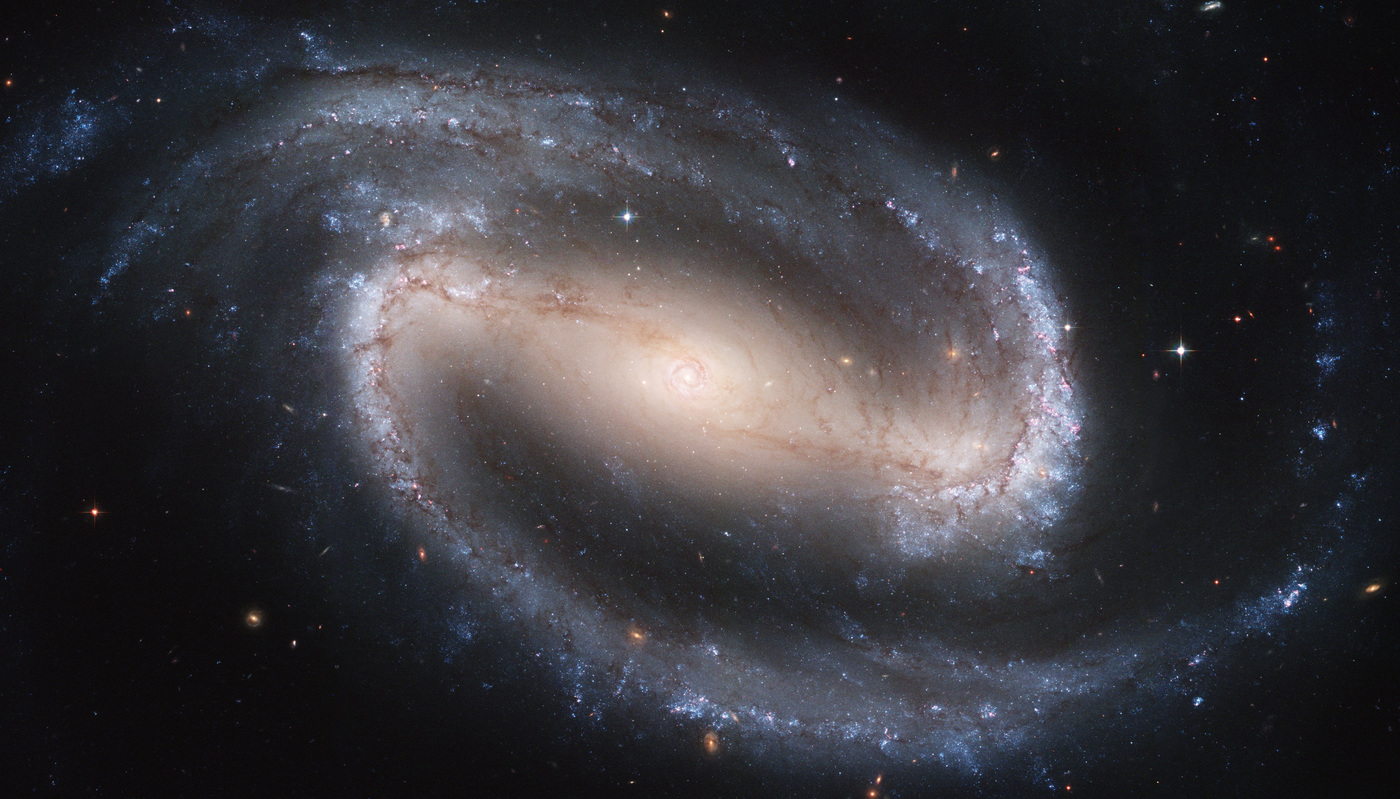
\includegraphics[width=0.99\columnwidth]{images/NGC1300.jpg}\caption{Спиральная галактика (<<туманность>>) с перемычкой (NGC 1300)}\end{figure}}
\vs p015 5:6 \li{4.}\bibemph{Центробежные планетарные дочери}. На определённых стадиях своего развития и в случае значительного увеличения частоты вращения, огромные солнца начинают выбрасывать в больших количествах материю, впоследствии соединяющуюся в небольшие миры, которые продолжают обращаться вокруг материнского солнца.
\vs p015 5:7 \li{5.}\bibemph{Сферы гравитационной недостаточности}. Существует критический предел размера отдельных звёзд. Если, достигнув такого предела, солнце не замедляет своего вращения, оно обречено на расщепление; происходит деление солнца, и рождается новая двойная звезда этой разновидности. В результате такого гигантского разрушения впоследствии могут образоваться многочисленные малые планеты.
\vs p015 5:8 \li{6.}\bibemph{Звёзды, образовавшиеся в результате сжатия} [\bibemph{Contractural Stars}]. В малых системах самая большая внешняя планета иногда притягивает к себе соседние миры, в то время как планеты, близко расположенные к солнцу, начинают своё терминальное падение\fnst{То есть падение на центральную звезду, которое завершает их существование в качестве планет.}. В случае вашей солнечной системы такой конец означал бы, что четыре внутренних планеты были бы поглощены солнцем, в то время как крупнейшая планета --- Юпитер --- сильно увеличилась бы за счёт захвата остальных миров. Такой конец солнечной системы привёл бы к образованию двух соседних, но неравных солнц, как одного из типов образования двойной звезды. Такие катастрофы случаются нечасто, за исключением периферии звёздных скоплений сверхвселенной.
\vs p015 5:9 \li{7.}\bibemph{Кумулятивные\fnst{То есть возникающие за счёт накопления --- аккумуляции --- материи.} сферы}. Из огромного количества материи, циркулирующей в пространстве, могут медленно накапливаться маленькие планеты. Они растут за счёт метеорной аккреции\fnst{В астрофизике под <<аккрецией>> понимают захват (обычно гравитационный) вещества каким\hyp{}либо массивным телом, например: аккреция газа нейтронной звездой с поверхности обычной звезды\hyp{}компаньона.} и незначительных столкновений. В определённых секторах пространства условия благоприятствуют таким формам планетарного рождения. Многие обитаемые миры имели такое происхождение.
\vs p015 5:10 Некоторые плотные тёмные острова являются прямым результатом аккреции преобразующейся в пространстве энергии. Другая группа таких тёмных островов возникла в результате скопления огромного количества холодной материи --- циркулирующих в пространстве осколков и метеоров. Такие скопления материи никогда не были горячими и, за исключением плотности, по составу очень похожи на Урантию.
\vs p015 5:11 \li{8.}\bibemph{Выгоревшие солнца}. Некоторые из тёмных островов пространства --- это выгоревшие изолированные солнца, излучившие всю доступную пространственную энергию. Такие организованные единицы материи приближаются к полной конденсации, почти полному затвердеванию; и потребуются многие эпохи для того, чтобы такие огромные массы сверхплотной материи могли перезарядиться в контурах пространства и подготовиться к новым циклам функционирования во вселенной после столкновения или другого возрождающего к жизни космического события.
\vs p015 5:12 \li{9.}\bibemph{Коллизионные\fnst{От лат. collisio: <<столкновение>>.} сферы}. В областях более плотного скопления столкновения --- не редкость. Такое астрономическое перестраивание сопровождается колоссальными изменениями энергии и преобразованиями материи. Особенно столкновения, в которых участвуют потухшие [dead] солнца, вызывают широкомасштабные флуктуации энергии. Возникающие после столкновения обломки часто образуют материальные ядра для последующего формирования планетарных тел, приспособленных для обитания смертных.
\vs p015 5:13 \li{10.}\bibemph{Архитектурные миры}. Это миры, которые построены в соответствии с планами и особенностями для некоторой специальной цели, такие как Салвингтон\fnst{Синтетическое слово. Возможно, от английского salvation $+$ town, что в переводе значит: <<город спасения>> или <<город, связанный со Спасителями>>.}, центр вашей локальной вселенной, и Уверса, место пребывания правительства нашей сверхвселенной.
\vs p015 5:14 \pc Существует множество других методов эволюции солнц и отделения планет, но именно с помощью вышеизложенных методов возникает подавляющее большинство звёздных систем и планетарных семейств. Для описания всего разнообразия методов, задействованных в звёздных метаморфозах и эволюции планет, потребовалось бы рассказать о почти 100 различных способах солнцеобразования и возникновения планет. Ваши астрономы [star students], сканируя небеса, обнаружат явления, указывающие на все эти способы звёздной эволюции, но им редко удастся заметить признаки формирования тех небольших несветящихся скоплений материи, которые служат в качестве обитаемых планет, --- самых важных из многочисленных материальных творений\fnst{Первая планета, находящаяся за пределами Солнечной системы (<<экзопланета>>), была открыта в 1988 году, и с тех пор их число удваивается примерно каждые 27 месяцев. По состоянию на 9~мая 2021 года подтверждено существование 4723 экзопланет в 3493 планетных системах, из которых в 773 имеется более одной планеты.}.
\usection{СФЕРЫ ПРОСТРАНСТВА}
\vs p015 6:1 Независимо от происхождения, различные сферы пространства можно разделить на следующие основные подразделения:
\vs p015 6:2 \li{1.}Солнца --- звёзды пространства.
\vs p015 6:3 \li{2.}Тёмные острова пространства.
\vs p015 6:4 \li{3.}Малые тела пространства\fnst{Или <<космические тела>>.} --- кометы, метеоры и планетезимали.
\vs p015 6:5 \li{4.}Планеты, включая обитаемые миры.
\vs p015 6:6 \li{5.}Архитектурные сферы --- специально созданные миры.
\vs p015 6:7 \pc За исключением архитектурных сфер, все космические тела имеют эволюционное происхождение, эволюционное в том смысле, что они не появились в результате прямого акта Божества; и в том, что созидательные акты Бога были раскрыты посредством время\hyp{}пространственного метода через действия многих созданных и возникших разумных существ Божества.
\vs p015 6:8 \pc \bibemph{Солнца}. Это звёзды пространства на всех различных стадиях их существования. Одни из них --- одиночные эволюционирующие системы в пространстве; другие представляют собой двойные звёзды, сжимающиеся или исчезающие планетарные системы. Звёзды пространства существуют не менее чем в тысяче различных состояний и стадий. Вы знакомы с солнцами, которые излучают свет, сопровождаемый теплом; но существуют солнца, которые светят без тепла.
\vs p015 6:9 Триллионы и триллионы лет, в течение которых обычное солнце будет продолжать выделять тепло и свет, хорошо иллюстрируют колоссальный запас энергии, который содержится в каждой единице материи. Фактическая энергия, запасённая в этих невидимых частицах физической материи, почти невообразима. И почти вся эта энергия под воздействием огромного теплового давления и связанной с этим энергетической активностью, преобладающей внутри пылающих солнц, выделяется в виде света. Другие условия позволяют этим солнцам преобразовывать и излучать значительную часть той энергии пространства, которая достигает их по установленным пространственным контурам. Многие фазы физической энергии и все формы материи притягиваются и впоследствии распределяются солнечными генераторами. Таким образом, солнца служат в качестве локальных ускорителей циркуляции энергии, действуя как станции автоматического регулирования мощи.
\vs p015 6:10 Сверхвселенная Орвонтон освещается и обогревается более чем десятью триллионами пылающих солнц. Эти солнца --- звёзды доступной вашему обозрению астрономической системы. Более двух триллионов солнц слишком далеки и слишком малы, чтобы быть видимыми с Урантии. Но в главной вселенной столько же солнц, сколько стаканов воды в океанах вашего мира\fnst{В океанах Урантии примерно $10^{21}$ стаканов воды, а в нашей Галактике около $10^{11}$ звёзд. Следовательно, главная вселенная содержит приблизительно десять миллиардов галактик, размером с Млечный Путь.}.
\vs p015 6:11 \pc \bibemph{Тёмные острова пространства}. Это потухшие солнца и другие крупные скопления материи, лишённые света и тепла. Тёмные острова иногда обладают огромной массой и оказывают сильное влияние на равновесие во вселенной и на управление энергией. Плотность некоторых из этих больших масс почти невероятна. И эта огромная концентрация массы позволяет тёмным островам действовать в качестве мощного балансира, удерживая в надёжной узде большие соседние с ними системы. Они поддерживают гравитационный баланс мощи во многих созвездиях; многие физические системы, которым в противном случае грозило бы быстрое погружение в соседние солнца и разрушение, надёжно удерживаются гравитационным охватом этих тёмных островов\hyp{}хранителей. Именно благодаря этой функции мы можем точно определять их местонахождение. Мы измерили гравитационное притяжение светящихся тел, что позволяет вычислить точный размер и расположение тёмных островов пространства, столь эффективно поддерживающих устойчивость данной системы на её пути.
\vs p015 6:12 \pc \bibemph{Малые тела пространства}. Метеоры и другие мелкие частицы материи, циркулирующие и эволюционирующие в пространстве, составляют огромную совокупность энергии и материальной субстанции.
\vs p015 6:13 Многие кометы --- это неустановившееся, неуправляемое [wild] потомство солнечных материнских дисков, постепенно переходящее под контроль центрального управляющего солнца. Кометы имеют также и различные другие виды происхождения. Хвост кометы направлен в противоположную сторону от притягивающего тела или солнца из\hyp{}за электрической реакции его сильно разрежённых газов и фактического давления света и других энергий, излучаемых солнцем. Это явление служит одним из убедительных доказательств реальности света и связанных с ним энергий; оно демонстрирует то, что свет имеет вес. Свет --- это реальная субстанция, а не просто волны гипотетического эфира.
\vs p015 6:14 \pc \bibemph{Планеты}. Это более крупные скопления материи, движущиеся по орбите вокруг солнца или другого космического тела; они варьируются по размеру от планетезималей до огромных газообразных, жидких или твёрдых сфер. Холодные миры, построенные в результате скопления летающего в пространстве вещества, становятся наиболее идеальными планетами для разумных обитателей, когда оказываются в правильной взаимосвязи с ближайшим солнцем. Потухшие солнца, как правило, не приспособлены для жизни; они обычно слишком далеки от живых пылающих солнц и, кроме того, слишком массивны; гравитация на их поверхности огромна.
\vs p015 6:15 В вашей сверхвселенной менее чем одна из сорока холодных планет пригодна для обитания существами вашей категории. И конечно, сверхгорячие солнца и холодные отдалённые миры непригодны для высших форм жизни. В вашей солнечной системе только три планеты\fnst{Две другие планеты, пригодные для обитания в Солнечной системе: Марс и Венера. См.\,\cite{Eddington1}, стр.\,170.} в настоящее время пригодны для жизни. Урантия по своему размеру, плотности и местоположению во многих отношениях идеальна для обитания человека.
\vs p015 6:16 Законы поведения физической энергии в основном универсальны, но местные влияния связаны с физическими условиями, преобладающими на отдельных планетах и в локальных системах. Бесчисленные миры пространства характеризует почти бесконечное разнообразие жизни созданий и других живых проявлений. Однако есть определённые точки сходства в группе миров, объединённых в одну систему, а также существует вселенская модель разумной жизни. Существует физическая взаимосвязь планетарных систем, принадлежащих одному физическому контуру и тесно следующих друг за другом в бесконечном движении по кругу вселенных.
\usection{АРХИТЕКТУРНЫЕ СФЕРЫ}
\vs p015 7:1 Правительство каждой сверхвселенной осуществляет своё руководство, находясь рядом с центром эволюционных вселенных своего сегмента пространства, и занимает специально созданный мир, населённый аккредитованными личностями. Эти столичные миры представляют собой архитектурные сферы --- тела пространства, специально сконструированные для особой цели. Хотя эти сферы и пользуются светом близлежащих солнц, освещаются и обогреваются они независимо. Каждая имеет солнце, дающее свет без тепла, подобно спутникам Рая, и обогревается за счёт циркуляции определённых энергетических потоков около поверхности сферы. Эти столичные миры принадлежат к одной из крупнейших систем, расположенных вблизи астрономического центра соответствующих сверхвселенных.
\vs p015 7:2 \pc Время в столицах сверхвселенных стандартизировано. Стандартный день сверхвселенной Орвонтон равен почти 30 дням времени Урантии, а год Орвонтона равен 100 стандартным дням. Этот год Уверсы является стандартом для седьмой сверхвселенной, и он на 22 минуты короче 3\,000 дней урантийского времени, что составляет примерно 8,2 ваших лет.
\vs p015 7:3 \pc Столичные миры семи сверхвселенных сопричастны природе и величию Рая, их центральному образцу совершенства. В действительности все столичные миры раеподобны [paradisiacal]. Это поистине небесные обители, и они увеличиваются в материальных размерах, моронтийной красоте и духовной славе от Иерусема до центрального Острова. И все спутники столичных миров также являются архитектурными сферами.
\vs p015 7:4 В различных столичных мирах представлена каждая фаза материального и духовного творения. Все виды материальных, моронтийных и духовных существ чувствуют себя как дома на этих вселенских мирах встреч. По мере восхождения во вселенной, переходя от материальных миров к духовным, смертные никогда не теряют восприятия и наслаждения от своих прежних уровней существования.
\vs p015 7:5 \pc \bibemph{Иерусем,} столица вашей локальной системы Сатания, имеет семь миров переходной культуры, каждый из которых окружён семью спутниками, среди которых семь обительских миров моронтийного заключения\fnst{Использованное здесь английское слово \bibemph{detention} означает <<тюремное заключение, лишение свободы>>. Семь обительских миров являются местами временного заключения: свобода действий и передвижений бывших смертных ограничена до тех пор, пока истинные мотивы души восходящего смертного не будут установлены окончательно, то есть до момента слияния с духом Отца.}, --- первого места пребывания человека после смерти. Термин <<небеса>>, как он использовался на Урантии, иногда обозначал эти семь обительских миров; первый обительский мир назывался первым небом и так далее до седьмого.
\vs p015 7:6 \pc \bibemph{Эденция,} столица вашего созвездия Норлатиадек, имеет 70 спутников культуры социализации и воспитания, где идущие по пути восхождения пребывают после завершения иерусемского режима мобилизации, объединения и реализации личности.
\vs p015 7:7 \pc \bibemph{Салвингтон}, столица вашей локальной вселенной Небадон, окружён 10 группами университетов по 49 сфер в каждой. Здесь человек одухотворяется после своей социализации в созвездии.
\vs p015 7:8 \pc \bibemph{Уминор третий,} столица вашего малого сектора Энса, окружён семью сферами высших физических исследований восходящей жизни.
\vs p015 7:9 \pc \bibemph{Умажор пятый,} столица вашего большого сектора Спландон, окружён 70 сферами развивающей интеллектуальной подготовки сверхвселенной.
\vs p015 7:10 \pc \bibemph{Уверса,} столица вашей сверхвселенной Орвонтон, непосредственно окружена 7 высшими университетами углублённой духовной подготовки восходящих волевых созданий. Каждая из этих семи групп удивительных сфер состоит из 70 специализированных миров, содержащих тысячи и тысячи разнообразных учреждений и организаций, посвящённых вселенскому образованию и культуре духа, где пилигримы времени переобучаются и переэкзаменуются перед своим долгим полётом к Хавоне. Прибывающие пилигримы времени всегда принимаются на этих вспомогательных мирах, но отбывающие выпускники всегда отправляются в Хавону прямо с берегов Уверсы.
\vs p015 7:11 Уверса является духовным и административным центром примерно одного триллиона обитаемых или пригодных для обитания миров. Слава, величие и совершенство столицы Орвонтона превосходит любое из чудес время\hyp{}пространственных творений.
\vs p015 7:12 \pc Если бы все спроектированные локальные вселенные и их составные части уже существовали, то в семи сверхвселенных было бы чуть менее 500 миллиардов\fnst{Точное число --- 453\,313\,764\,407. Оно вычисляется следующим образом: 7\dt(1+7\dt70+10\dt(70+1)+1000\dt(7+1)+100\,000\dt647\,591).} архитектурных миров.
\usection{КОНТРОЛЬ И РЕГУЛИРОВАНИЕ ЭНЕРГИИ}
\vs p015 8:1 Столичные сферы сверхвселенных сконструированы так, что могут функционировать как эффективные регуляторы мощи\hyp{}энергии для соответствующих секторов, выступая в качестве фокальных точек для направления энергии в составляющие их локальные вселенные. Они оказывают мощное влияние на баланс и управление физическими энергиями, циркулирующими в организованном пространстве.
\vs p015 8:2 Дальнейшие регулирующие функции выполняются центрами мощи и физическими регуляторами, живыми и полуживыми разумными сущностями, созданными для этой конкретной цели. Эти центры мощи и регуляторы трудны для понимания; низшие категории неспособны к принятию волевых решений, они не обладают волей, они не выбирают, их функции очень разумны, но, по\hyp{}видимому, автоматичны и свойственны их высокоспециализированной организации. Центры мощи и физические регуляторы сверхвселенных принимают на себя руководство и частичный контроль над 30 энергетическими системами, составляющими область гравиты. Чтобы завершить окружение сверхвселенной контурами физической энергии, управляемые центрами мощи Уверсы, требуется немногим более 968\,000\,000 лет.
\vs p015 8:3 \pc Развивающаяся энергия обладает субстанцией; она имеет вес, хотя вес всегда относителен и зависит от скорости обращения, массы и антигравитации. Масса в материи стремится замедлять скорость в энергии\fnst{Если рассматривать массу покоя $m$ как канонический импульс $p^5=m$ в 5\hyp{}мерном пространстве, сопряжённый собственному времени $\tau$ (или интервалу, играющему роль действия для свободной частицы), то это иначе бессмысленное утверждение становится почти понятным. См.\,\bibref[23:3.2]{p023 3:3}.}; а присутствующая повсюду скорость энергии представляет собой: начальное значение скорости минус замедление, вызванное массой во время перемещения, плюс регулирующую функцию живых регуляторов энергии сверхвселенной и физическое влияние близлежащих сильно нагретых или тяжело заряженных [heavily charged] тел.
\vs p015 8:4 Универсальный план поддержания равновесия между материей и энергией требует постоянного создания и разрушения малых материальных единиц. Управляющие Вселенской Мощью обладают способностью уплотнять и удерживать или расширять и высвобождать различные количества энергии.
\vs p015 8:5 При достаточно продолжительном замедляющем влиянии, гравитация в конце концов преобразовала бы всю энергию в материю, если бы не два фактора: во\hyp{}первых, антигравитационное влияние регуляторов энергии, и, во\hyp{}вторых, тенденция к распаду организованной материи при определённых условиях, встречающихся в очень горячих звёздах, и при особых условиях в пространстве вблизи высокоэнергетических холодных тел из сжатой [condensed] материи.
\vs p015 8:6 Когда масса становится сверхагрегированной и угрожает нарушить баланс энергию, истощить контуры физической мощи, вмешиваются физические регуляторы, если только дальнейшая тенденция гравитации к чрезмерной материализации энергии не прекратится из\hyp{}за случайного столкновения между мёртвыми гигантами космоса, тем самым, мгновенно рассеивая кумулятивные скопления гравитации. В случае таких столкновений огромные массы материи внезапно превращаются в редчайшую форму энергии, и борьба за всеобщее равновесие начинается снова. В итоге более крупные физические системы стабилизируются, становятся физически устойчивыми и включаются в сбалансированные и установившиеся контуры сверхвселенных. После этого события в таких устойчивых системах больше не происходит столкновений или других разрушительных катастроф.
\vs p015 8:7 В периоды избытка энергии наблюдаются энергетические возмущения и тепловые флуктуации, сопровождаемые электрическими феноменами. В периоды недостатка энергии возрастают тенденции материи к накоплению, уплотнению и выходу из\hyp{}под контроля в более тонко сбалансированных контурах; возникающие вследствие этого приливные или коллизионные изменения быстро восстанавливают баланс между циркулирующей энергией и, буквально, более стабильной материей. Прогнозирование и понимание такого вероятного поведения пылающих солнц и тёмных островов пространства --- одна из задач небесных наблюдателей звёзд.
\vs p015 8:8 Мы способны распознать большинство законов, управляющих вселенским равновесием, и предсказать многое, относящееся к стабильности вселенной. На практике наши прогнозы надёжны, но мы постоянно сталкиваемся с определёнными силами, которые не полностью подчиняются известным нам законам управления энергией и поведения материи. По мере нашего продвижения из Рая наружу во вселенные, предсказуемость всех физических явлений затрудняется. Выходя за пределы личного управления Райских Правителей, мы сталкиваемся с растущей неспособностью производить расчёты в соответствии с установленными стандартами и опытом, приобретённым при наблюдениях, имеющих отношение исключительно к физическим явлениям ближайших астрономических систем. Даже в областях семи сверхвселенных мы живём в среде силовых воздействий и энергетических реакций, наполняющих все наши сферы и простирающихся в едином равновесии во все регионы внешнего пространства.
\vs p015 8:9 Чем дальше мы идём, тем больше вероятность столкновения с изменчивыми и непредсказуемыми явлениями, которые столь безошибочно характерны для непостижимого присутствия\hyp{}действия Абсолютов и эмпирических Божеств. И эти явления должны указывать на некий универсальный сверхконтроль над всеми вещами.
\vs p015 8:10 Сверхвселенная Орвонтон в настоящее время очевидно останавливается; внешние вселенные, кажется, заряжаются для беспрецедентной будущей активности; центральная вселенная Хавона вечно стабилизирована. Гравитация и отсутствие тепла (холод) организуют и скрепляют материю; тепло и антигравитация разрушают материю и рассеивают энергию. Живые управляющие мощью и организаторы силы --- вот секрет особого управления и разумного руководства бесконечными метаморфозами создания, разрушения и воссоздания вселенных. Туманности могут рассеиваться, солнца выгорать, системы исчезать, планеты погибать, но вселенные не останавливаются.
\usection{КОНТУРЫ СВЕРХВСЕЛЕННЫХ}
\vs p015 9:1 
\vs p015 9:2 
\vs p015 9:3 \pc 
\vs p015 9:4 
\vs p015 9:5 
\vs p015 9:6 
\vs p015 9:7 
\vs p015 9:8 
\vs p015 9:9 
\vs p015 9:10 
\vs p015 9:11 \pc 
\vs p015 9:12 
\vs p015 9:13 
\vs p015 9:14 
\vs p015 9:15 \pc 
\vs p015 9:16 
\vs p015 9:17 
\vs p015 9:18 \pc 
\usection{Rulers of the Superuniverses}
\vs p015 10:1 
\vs p015 10:2 
\vs p015 10:3 \pc 
\vs p015 10:4 
\vs p015 10:5 
\vs p015 10:6 
\vs p015 10:7 
\vs p015 10:8 
\vs p015 10:9 
\vs p015 10:10 
\vs p015 10:11 \pc 
\vs p015 10:12 
\vs p015 10:13 
\vs p015 10:14 
\vs p015 10:15 
\vs p015 10:16 
\vs p015 10:17 
\vs p015 10:18 
\vs p015 10:19 
\vs p015 10:20 
\vs p015 10:21 \pc 
\vs p015 10:22 \pc 
\vs p015 10:23 
\usection{The Deliberative Assembly}
\vs p015 11:1 
\vs p015 11:2 
\vs p015 11:3 
\usection{The Supreme Tribunals}
\vs p015 12:1 
\vs p015 12:2 
\vs p015 12:3 
\vs p015 12:4 
\usection{The Sector Governments}
\vs p015 13:1 
\vs p015 13:2 
\vs p015 13:3 
\vs p015 13:4 \pc 
\vs p015 13:5 
\vs p015 13:6 
\usection{Purposes of the Seven Superuniverses}
\vs p015 14:1 
\vs p015 14:2 
\vs p015 14:3 
\vs p015 14:4 
\vs p015 14:5 \pc 
\vs p015 14:6 
\vs p015 14:7 
\vs p015 14:8 
\vs p015 14:9 \pc 
\vsetoff
\vs p015 14:10 
\quizlink
\begin{thebibliography}{100}
\bibitem{Eddington1}
Sir Arthur Stanley Eddington.
{<<The Nature of the Physical World>>.}
{\em Cambridge, England}, 1929.
\end{thebibliography}
